% ---------------------------------------------------------------------------------------------------------
% Core domain: original (spider_web_htn) and config-driven "updated" (spider_web_htn_updated) HTN model.
% Figures: figures/core/*.{pdf,png}; scripts: scripts/core/; manifest: figures/core/MANIFEST.md
% ---------------------------------------------------------------------------------------------------------
\section{Progress on the Core HTN Model since Checkpoint 2}
\label{sec:core}

This section reports what the repository now contains for the two planners of Zschokke's \cite{zschokke1996early} construction sequence described in
Sections 1--10 of the Checkpoint 2 report: the original GTPyhop model (\texttt{spider\_web\_htn}) and the
config-driven model (\texttt{spider\_web\_htn\_updated}). Two kinds of evidence are kept apart throughout,
as the repository's claim ledger requires (claim C17: original and updated HTN evidence need separate
audit before any synthesis). \emph{Plans and geometry} are reported for the current code at commit
\texttt{61d18d8}. \emph{Sweep results} (\texttt{sensitivity\_comparison.csv},
\texttt{wind\_sensitivity.csv}, \texttt{single\_run\_comparison.csv}) were committed on 2026-09-09 at
commit \texttt{39b89f3} and were produced by the model as it was then (with the pre-November spiral
rule); they are reported as results of that version and are not merged with the current plan. Where we
re-ran code to check or extend a committed result, we did so in a private checkout at the stated commit
and say so; all scripts are listed in \texttt{figures/core/MANIFEST.md}.

% =========================================================================================================
\subsection{Which plan Checkpoint 2 showed, and what has changed}
\label{sec:core-plans}

Three different deterministic plans exist for the default rig, and the Checkpoint 2 report mixes two of
them. Table~\ref{tab:core-phases} and Figures~\ref{fig:core-webs}--\ref{fig:core-phases} put them side
by side.

\begin{itemize}
  \item \textbf{Checkpoint 2 plan} --- the updated package at \texttt{39b89f3} with stochasticity
  disabled: 71 actions, 600.1\,cm. This is the source of the 600.1\,cm total and the per-phase energies
  in Table 3 of the Checkpoint 2 report (that commit's own regression test,
  \texttt{tests/test\_planner.py}, asserts 71 actions and 600.1\,cm; the report prints 70 actions and 9
  exploration actions, which we could not reproduce from any committed code). Its ``spirals'' are a
  single anchor-to-anchor pass through the seven boundary anchors listed in
  \texttt{config.yaml:domain.spiral\_nodes}, i.e.\ a heptagon on the rig itself; the auxiliary and
  capture passes cover the same polygon in opposite directions (Figure~\ref{fig:core-webs}, left).
  \item \textbf{Original package} (\texttt{spider\_web\_htn}, unchanged since 2026-09-04): 128 actions,
  751.6\,cm. Its spirals step through interpolated radius points
  (\texttt{get\_radius\_node(anchor, frac)}), 4 turns $\times$ 8 anchors outward from $0.20$ to $0.80$ of
  the hub--anchor distance and 5 turns $\times$ 8 inward from $0.85$ to $0.20$. This is the procedure
  Algorithm 8 of the Checkpoint 2 report describes, and it is the plan the committed
  \texttt{visualization/index.html} has always displayed (\texttt{plan\_data.js}: 128 steps,
  751.6\,cm; Figure~\ref{fig:core-ui}a). The 70-action screenshot used as Figure 1 of the Checkpoint 2
  report cannot be regenerated from any committed data file.
  \item \textbf{Updated package at \texttt{61d18d8}} (current): 105 actions, 701.6\,cm. The first 52
  actions (exploration, proto-hub, frame, radii; 474.5\,cm) are identical to the Checkpoint 2 plan. Only
  the two spiral phases differ: the single heptagon pass is replaced by the multi-turn waypoint spirals of
  \texttt{spiral\_geometry.py} (Section~\ref{sec:core-spiral}), 20 auxiliary waypoints (22 actions with
  the return walk and marker; 86.5\,cm) and 28 capture waypoints (30 actions; 140.6\,cm). Hence
  $71 + 13 + 21 = 105$ actions and $600.1 + 23.7 + 77.8 = 701.6$\,cm.
\end{itemize}

\begin{table}[htbp]
\centering
\caption{Per-phase action counts and locomotory energy (Eq.~1 of the Checkpoint 2 report) of the three
deterministic default-rig plans. Exported by \texttt{scripts/core/export\_plan.py} in private checkouts
(Checkpoint 2 plan: updated package at \texttt{39b89f3}, \texttt{stochastic.enabled} forced to
\texttt{false}; the other two at \texttt{61d18d8}); phase tagging follows
\texttt{visualize\_updated.py}. Energies are unrounded sums; the Checkpoint 2 Table 3 values 84.0, 162.0
and 62.7 are sums of per-step values rounded to 0.1\,cm.}
\label{tab:core-phases}
\small
\begin{tabular}{lrrrrrr}
\toprule
 & \multicolumn{2}{c}{Checkpoint 2 plan} & \multicolumn{2}{c}{Original package} & \multicolumn{2}{c}{Updated package} \\
 & \multicolumn{2}{c}{(updated @ \texttt{39b89f3})} & \multicolumn{2}{c}{(\texttt{spider\_web\_htn})} & \multicolumn{2}{c}{(@ \texttt{61d18d8})} \\
\cmidrule(lr){2-3}\cmidrule(lr){4-5}\cmidrule(lr){6-7}
Phase & Actions & Energy (cm) & Actions & Energy (cm) & Actions & Energy (cm) \\
\midrule
Exploration \& bridging & 10 & 102.2 & 9 & 102.2 & 10 & 102.2 \\
Proto-hub establishment & 15 & 84.2 & 15 & 84.2 & 15 & 84.2 \\
Frame construction & 11 & 126.0 & 11 & 126.0 & 11 & 126.0 \\
Radii construction & 16 & 162.2 & 16 & 162.2 & 16 & 162.2 \\
Auxiliary spiral & 9 & 62.8 & 34 & 120.7 & 22 & 86.5 \\
Capture spiral & 9 & 62.8 & 42 & 156.5 & 30 & 140.6 \\
Finalisation & 1 & 0.0 & 1 & 0.0 & 1 & 0.0 \\
\midrule
Total & 71 & 600.1 & 128 & 751.6 & 105 & 701.6 \\
\bottomrule
\end{tabular}
\end{table}

\begin{figure}[htbp]
\centering
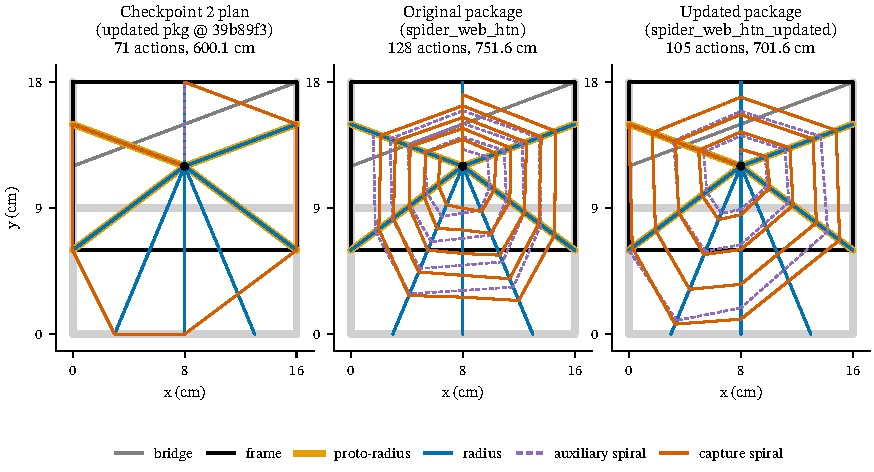
\includegraphics[width=\linewidth]{figures/core/web_final_three_plans}
\caption{Final simulated web of the three deterministic default-rig plans, drawn by replaying each plan's
actions with the thread semantics of the repository visualiser (\texttt{insert\_radius} turns a dragline
into a proto-radius). Light grey: the supporting rig (two 18\,cm sticks, bottom bar, crossbar). Proto-radii
(orange halo) coincide with the four lateral radii. In the Checkpoint 2 plan the auxiliary pass is hidden
under the capture pass, which retraces the same heptagon. All auxiliary-spiral threads remain in the model
state at completion (no plan contains \texttt{remove\_thread}). Note that the bottom frame thread runs
between the lower side anchors at $y=6$\,cm while three radii end on the bottom bar at $y=0$, so the web
extends below its own frame. $n=1$ plan each; sources: \texttt{visualization/plan\_data.js},
\texttt{visualization/plan\_data\_updated.js} and a re-export at \texttt{39b89f3}.}
\label{fig:core-webs}
\end{figure}

\begin{figure}[htbp]
\centering
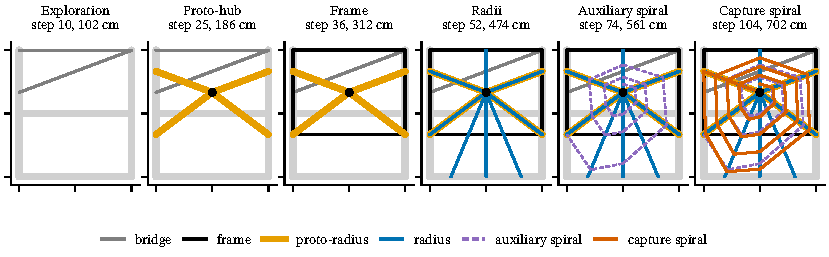
\includegraphics[width=\linewidth]{figures/core/web_buildup_updated}
\caption{Build-up of the current updated plan: the web after the last action of each macro phase, with the
step index and cumulative energy. Source: \texttt{visualization/plan\_data\_updated.js} (105 actions).}
\label{fig:core-buildup}
\end{figure}

Figure~\ref{fig:core-cumulative} redoes Figure 2 of the Checkpoint 2 report for the current plan. The
early and frame/radii phases are unchanged; what changed is the spiral part. In the Checkpoint 2 plan the
two spirals contributed 21.0\,\% of the energy; in the updated plan they contribute 32.3\,\%, and the
capture spiral alone (20.0\,\%) now costs almost as much as the radii (23.1\,\%). The earlier reading that
the spiral phases are ``comparatively shallow'' therefore described the heptagon placeholder rather than
a spiral. Two further details of the action counts follow from GTPyhop rather than from the domain:
GTPyhop~1.9.7 omits any action whose application leaves the state unchanged, so the
\textsc{Walk}$(h,h)$ ``circle the hub'' step of Algorithm 7 never appears in a plan, and the original
package's plan lacks \textsc{Attach-Dragline}, which is why its exploration phase has 9 actions rather
than 10.

\begin{figure}[htbp]
\centering
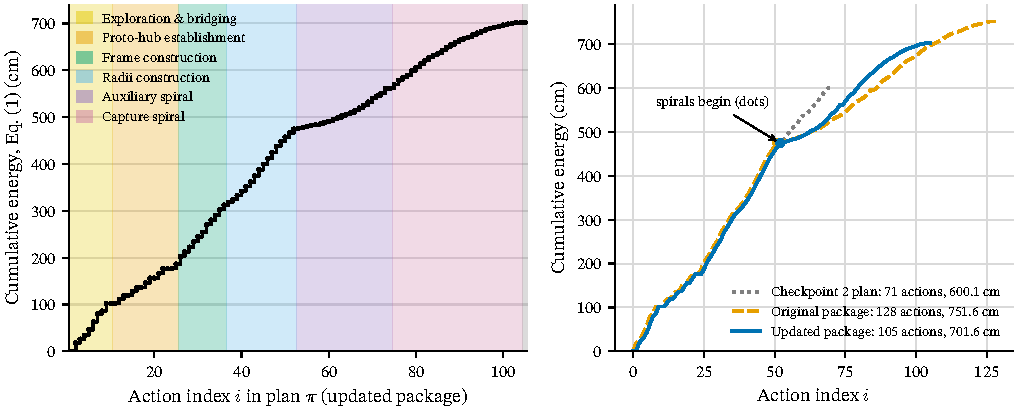
\includegraphics[width=\linewidth]{figures/core/energy_cumulative}
\caption{(a) Cumulative locomotory energy against action index for the current updated plan, shaded by
macro phase (counterpart of Checkpoint 2 Figure 2). Plateaus are zero-cost markers. (b) The three
plans overlaid; dots mark the first auxiliary-spiral action (step 52 or 53), after which the curves
separate. $n=1$ deterministic plan each; sources as Table~\ref{tab:core-phases}.}
\label{fig:core-cumulative}
\end{figure}

\begin{figure}[htbp]
\centering
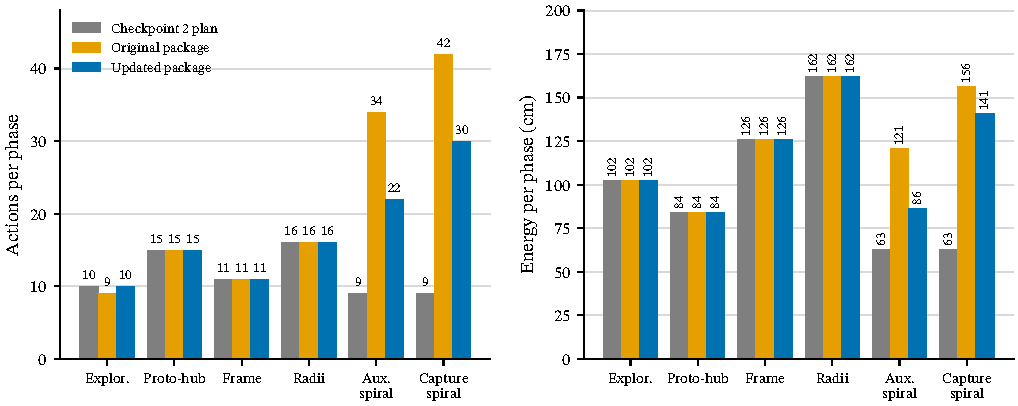
\includegraphics[width=\linewidth]{figures/core/energy_per_phase}
\caption{Actions (left) and locomotory energy (right) per macro phase for the three plans of
Table~\ref{tab:core-phases}. Only the spiral phases differ.}
\label{fig:core-phases}
\end{figure}

The interactive visualiser now exists in two versions (Figure~\ref{fig:core-ui}).
\texttt{visualization/index.html} plays the original package's plan; the new
\texttt{visualization/index\_updated.html} (added in \texttt{61d18d8}, generated by
\texttt{spider\_web\_htn\_updated/visualize\_updated.py}) plays the updated plan and labels the spirals
``log-spiral aux / Archimedean capture''. On reaching \texttt{mark\_web\_complete} the updated page stops
colour-coding, draws all threads as plain silk and hides the auxiliary spiral as removed scaffolding; this
is a display choice only, since the model keeps those threads and counts their energy.

\begin{figure}[htbp]
\centering
\begin{subfigure}[b]{0.49\linewidth}
  \centering
  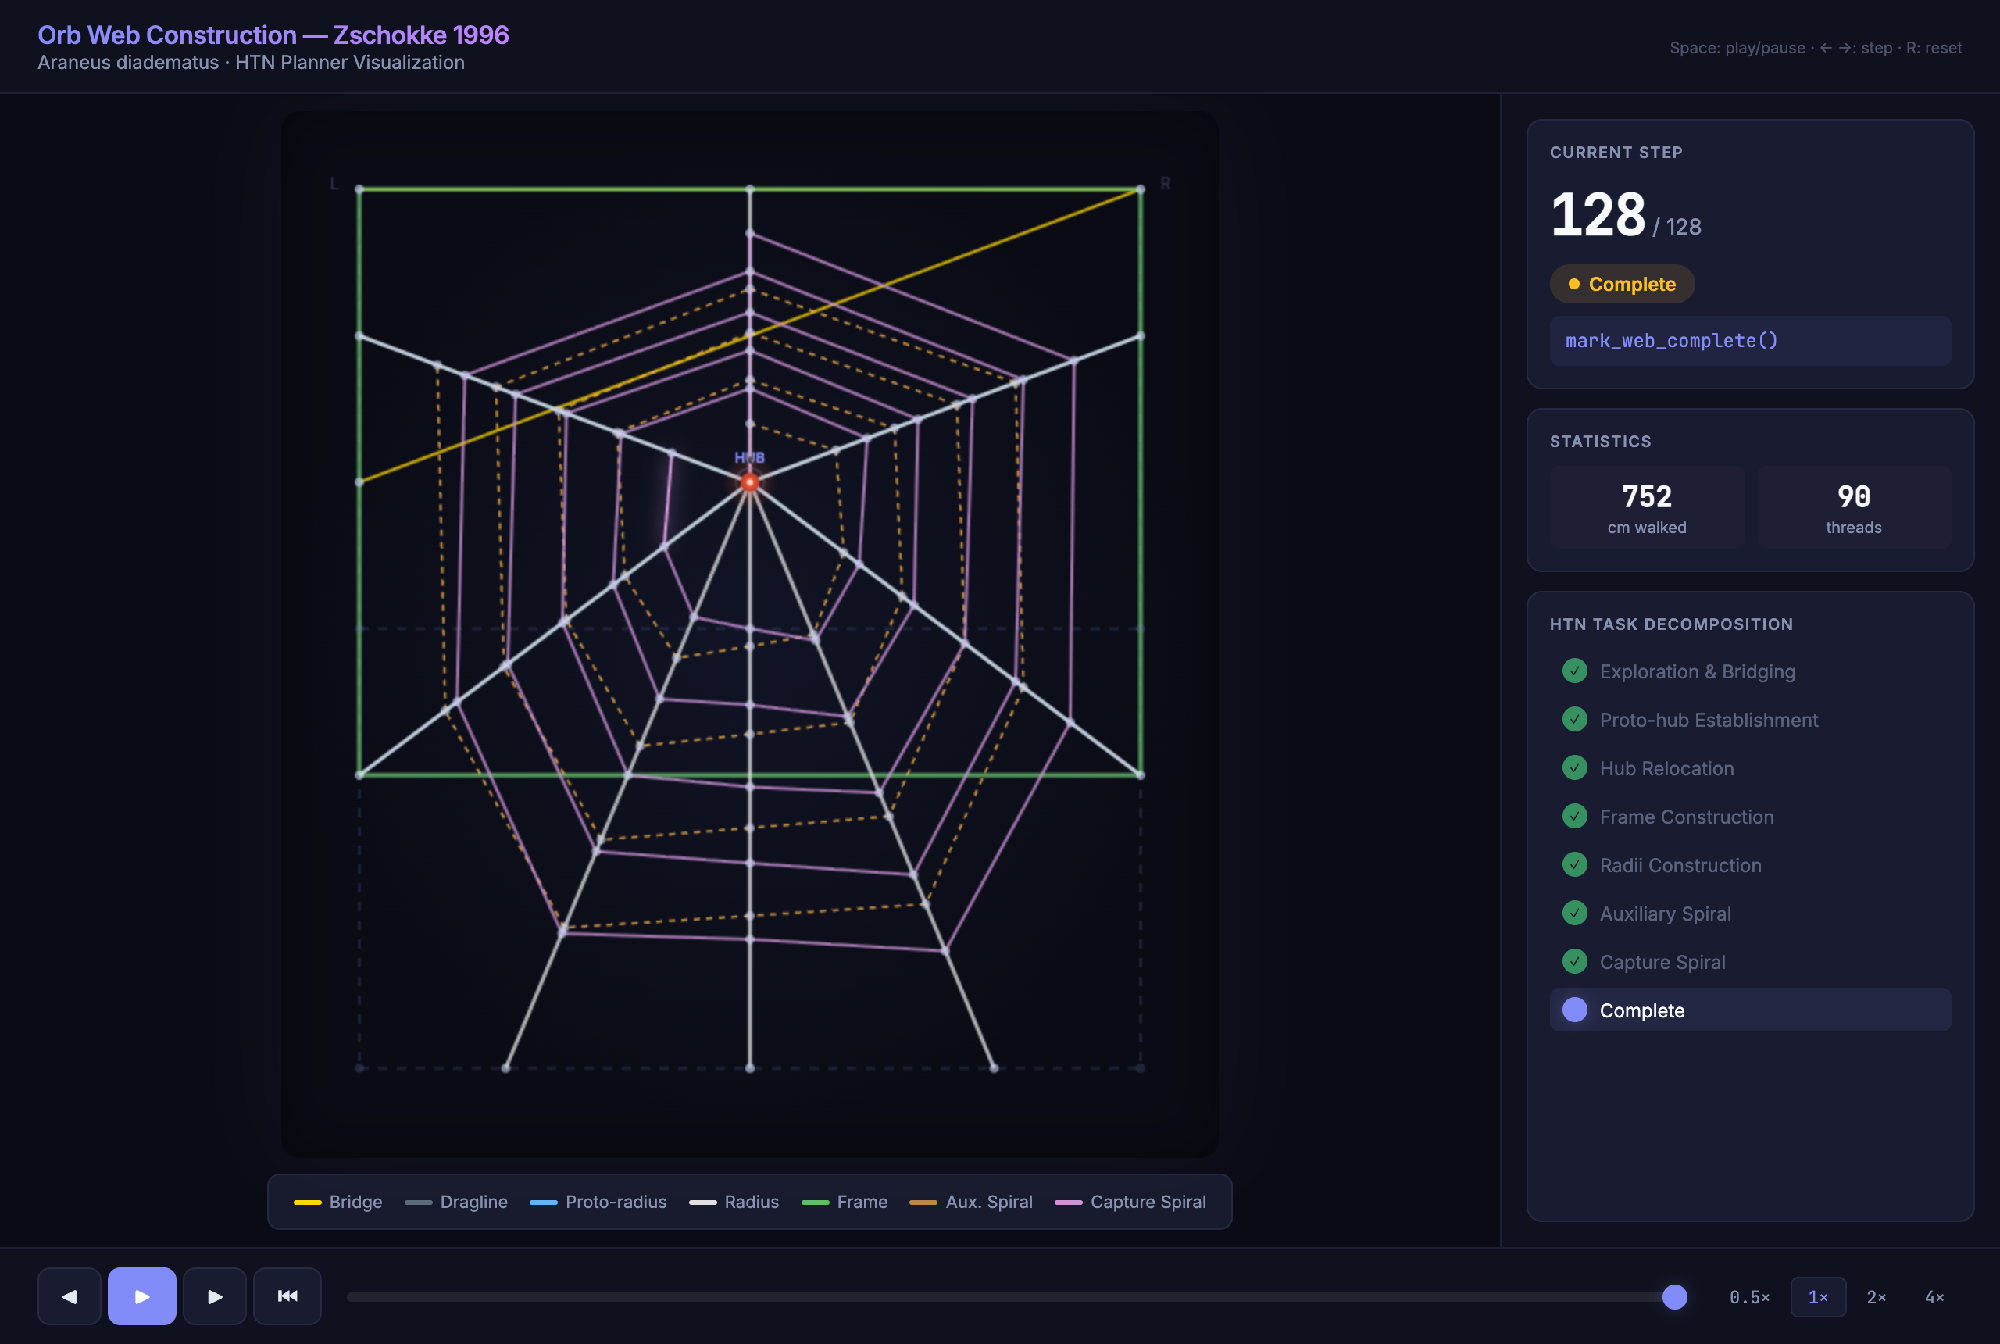
\includegraphics[width=\linewidth]{figures/core/ui_original_final}
  \caption{\texttt{index.html}, step 128/128}
\end{subfigure}\hfill
\begin{subfigure}[b]{0.49\linewidth}
  \centering
  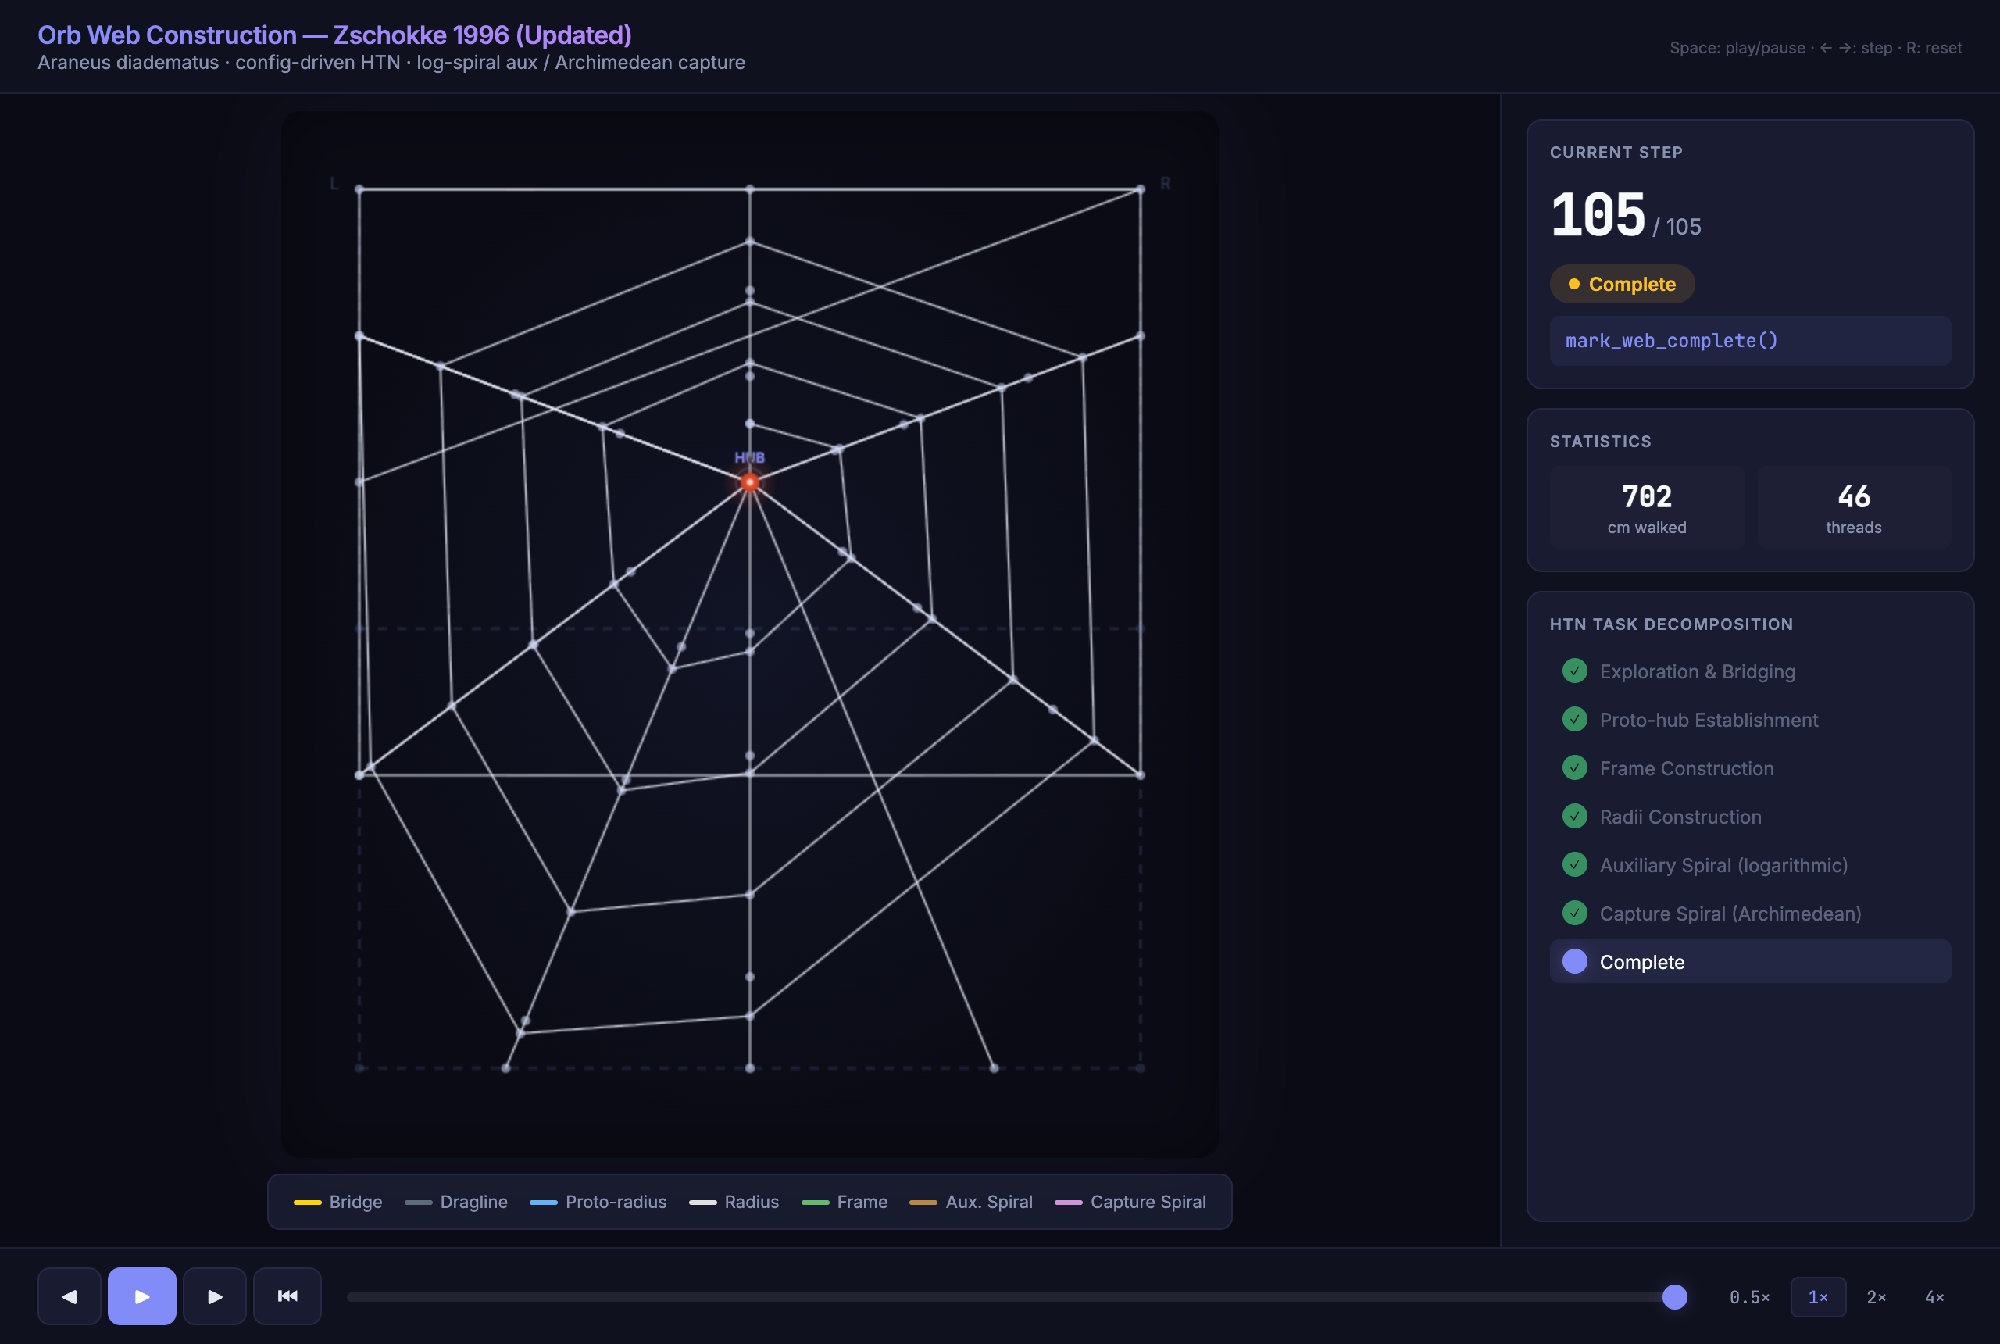
\includegraphics[width=\linewidth]{figures/core/ui_updated_final}
  \caption{\texttt{index\_updated.html}, step 105/105}
\end{subfigure}
\par\medskip
\begin{subfigure}[b]{0.49\linewidth}
  \centering
  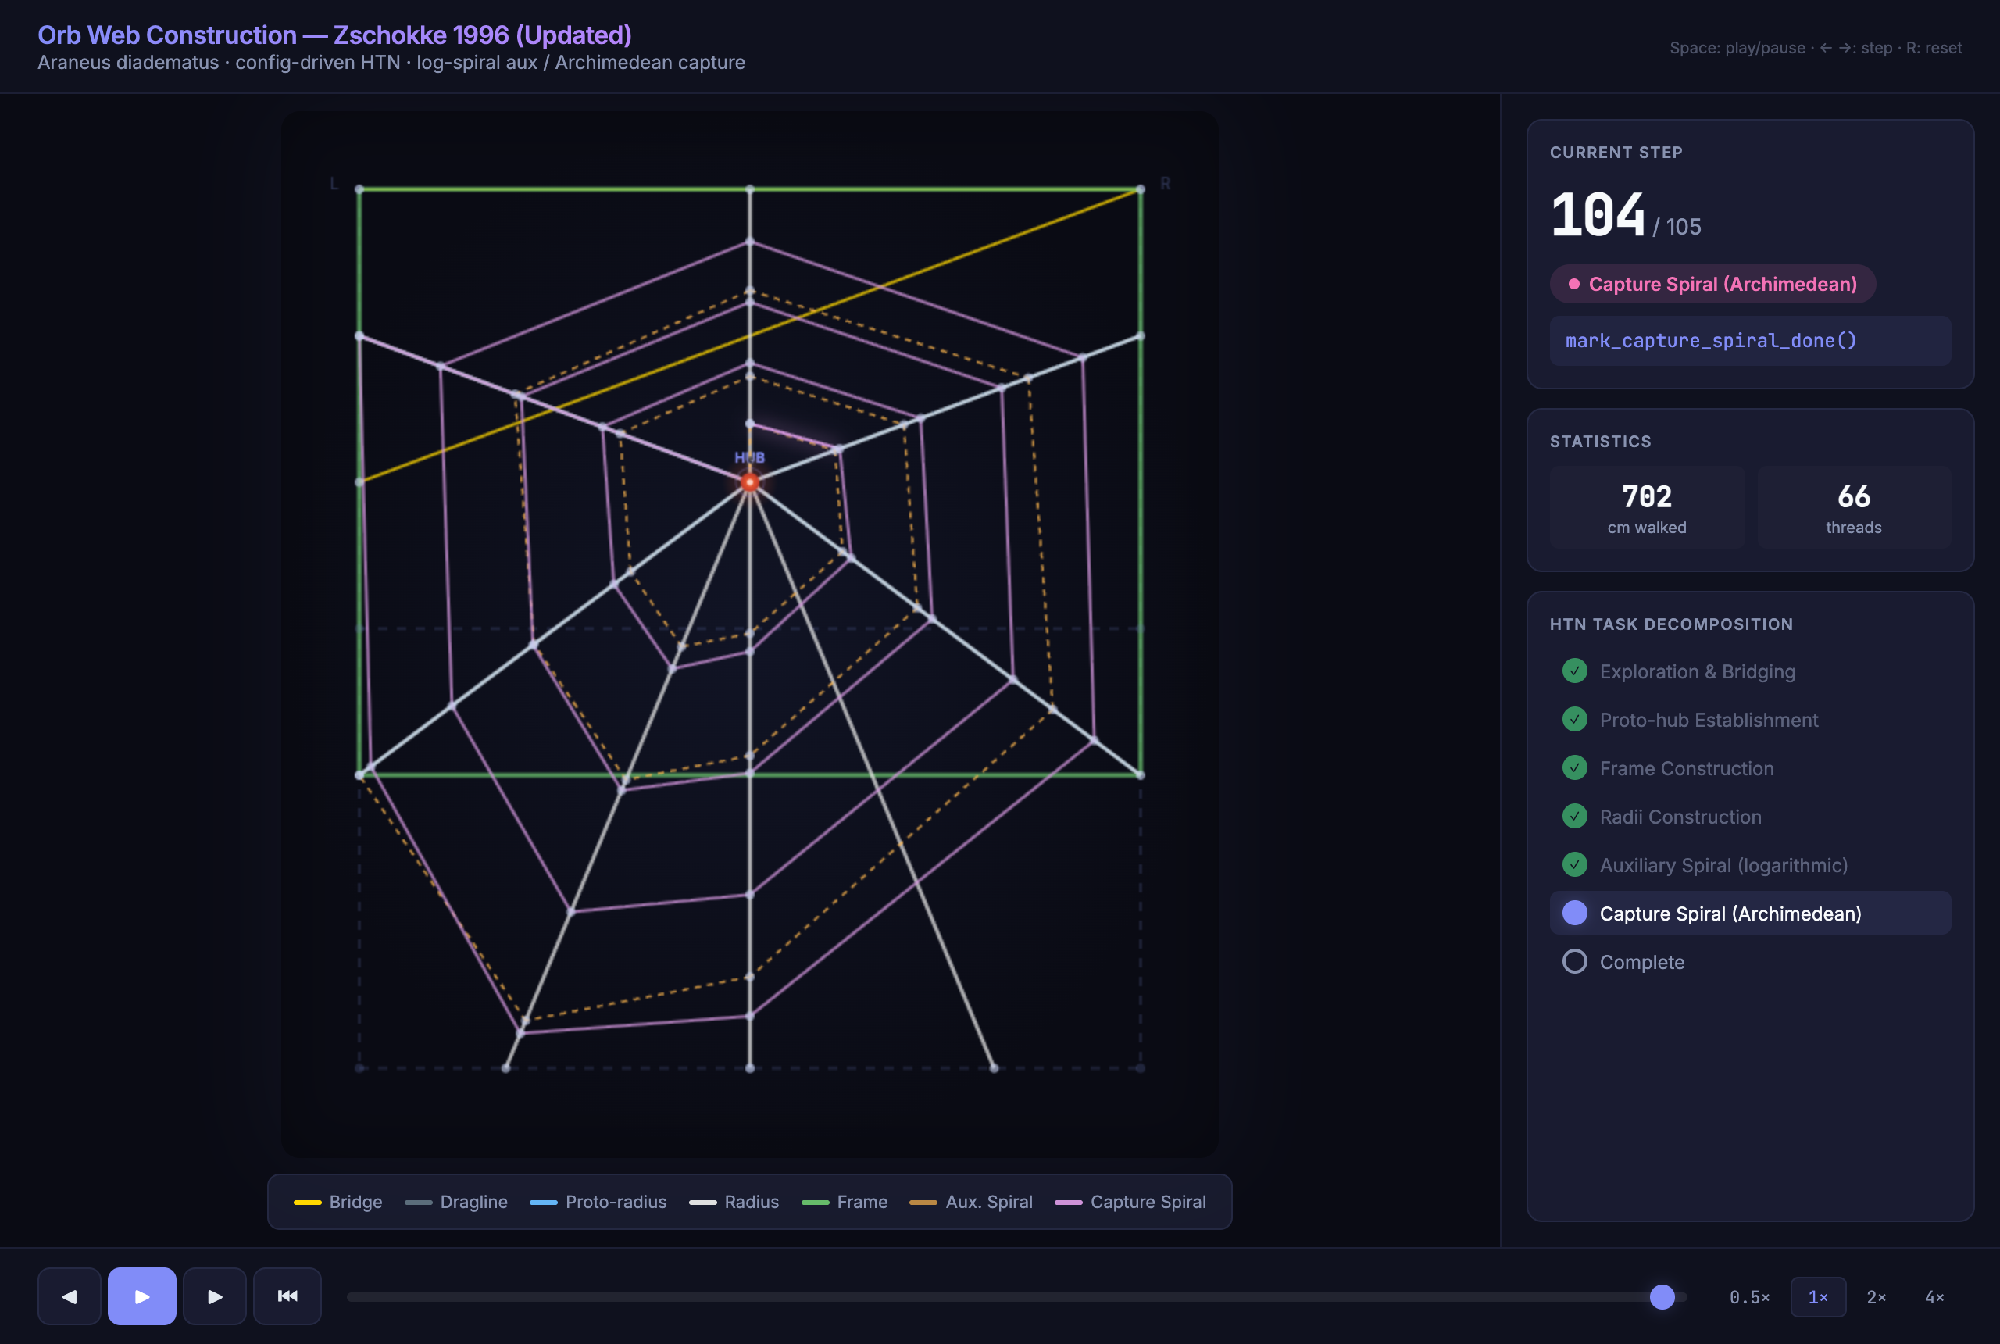
\includegraphics[width=\linewidth]{figures/core/ui_updated_precomplete}
  \caption{\texttt{index\_updated.html}, step 104 (before completion)}
\end{subfigure}
\caption{The repository's interactive plan visualisers, captured in headless Chrome after jumping to the
stated step (\texttt{scripts/core/capture\_ui.sh}). (a) Original package: 128 actions, 752\,cm walked,
90 threads. (b) Updated package at completion: 702\,cm, 46 threads drawn (auxiliary spiral hidden by the
page). (c) The same page one step earlier, still colour-coded (66 threads). Data:
\texttt{visualization/plan\_data.js} and \texttt{plan\_data\_updated.js} at \texttt{61d18d8}.}
\label{fig:core-ui}
\end{figure}

% =========================================================================================================

\subsection{Spiral geometry}
\label{sec:core-spiral}

\texttt{spiral\_geometry.py} replaces the heptagon pass with explicit polar waypoints around the hub $h$.
For the $D=7$ directions listed in \texttt{domain.spiral\_nodes} (each anchor $j$ gives an angle
$\theta_j$ and an outer radius $r_{T,j}=\lVert x_j - x_h\rVert$), waypoint $i=0,\dots,N-1$ belongs to
direction $j(i)=i \bmod D$, sits at angle $\theta_{j(i)} + 2\pi\lfloor i/D\rfloor$, and has
\begin{align}
  r_i^{\mathrm{aux}} &= (\rho\, r_{T,j})^{\,1-f_i}\; r_{T,j}^{\,f_i}, &
  r_i^{\mathrm{cap}} &= r_{T,j} - (1-\rho)\, r_{T,j}\, f_i, &
  f_i &= \frac{i}{N-1}, \label{eq:core-spiral}
\end{align}
i.e.\ geometric (logarithmic) outward growth for the auxiliary spiral and linear (Archimedean) inward decay
for the capture spiral, both between $\rho\,r_{T,j}$ and $r_{T,j}$ with
$\rho=$\,\texttt{start\_radius\_fraction}\,$=0.20$. $N$ is
$\mathrm{round}(\texttt{turns}\times\texttt{steps\_per\_turn})$: $2.5\times 8=20$ auxiliary and
$3.5\times 8=28$ capture waypoints. Each waypoint is skipped if its source anchor has been removed by the
stochastic layer. Figure~\ref{fig:core-spiral} shows the result and three properties that are visible only
in the generated geometry:
\begin{itemize}
  \item Because one rotation is $D=7$ waypoints, not \texttt{steps\_per\_turn}\,$=8$, the spirals make
  2.71 and 3.86 rotations rather than the configured 2.5 and 3.5.
  \item \texttt{anchor\_bottom\_right} is not in \texttt{spiral\_nodes}, so one of the eight radii carries
  no spiral waypoint and the spirals cut across that sector (panel a).
  \item The radial gap between successive loops on the same radius is 9.7--53.4\,mm for the auxiliary
  spiral (growing outward, as intended) and 12.4--27.0\,mm for the capture spiral (constant per direction).
  The configuration's \texttt{empirical.mesh\_size\_mm}\,$=2.33$ is not used by the geometry (panel c);
  the rig and the cited field webs differ in scale, so this is a description, not a calibration test.
\end{itemize}
The \texttt{config.yaml} comment records that $\rho$ was raised from 0.08 to 0.20 to stop the log spiral
``rushing'' to the edge in its last turn, at a cost of 666.9\,$\to$\,701.6\,cm. Our sweep of $\rho$
(Figure~\ref{fig:core-spiral}d) reproduces both values and shows total plan energy rising roughly linearly
from 656.2\,cm at $\rho=0.05$ to 794.2\,cm at $\rho=0.60$; the action count stays 105 throughout.

\begin{figure}[htbp]
\centering
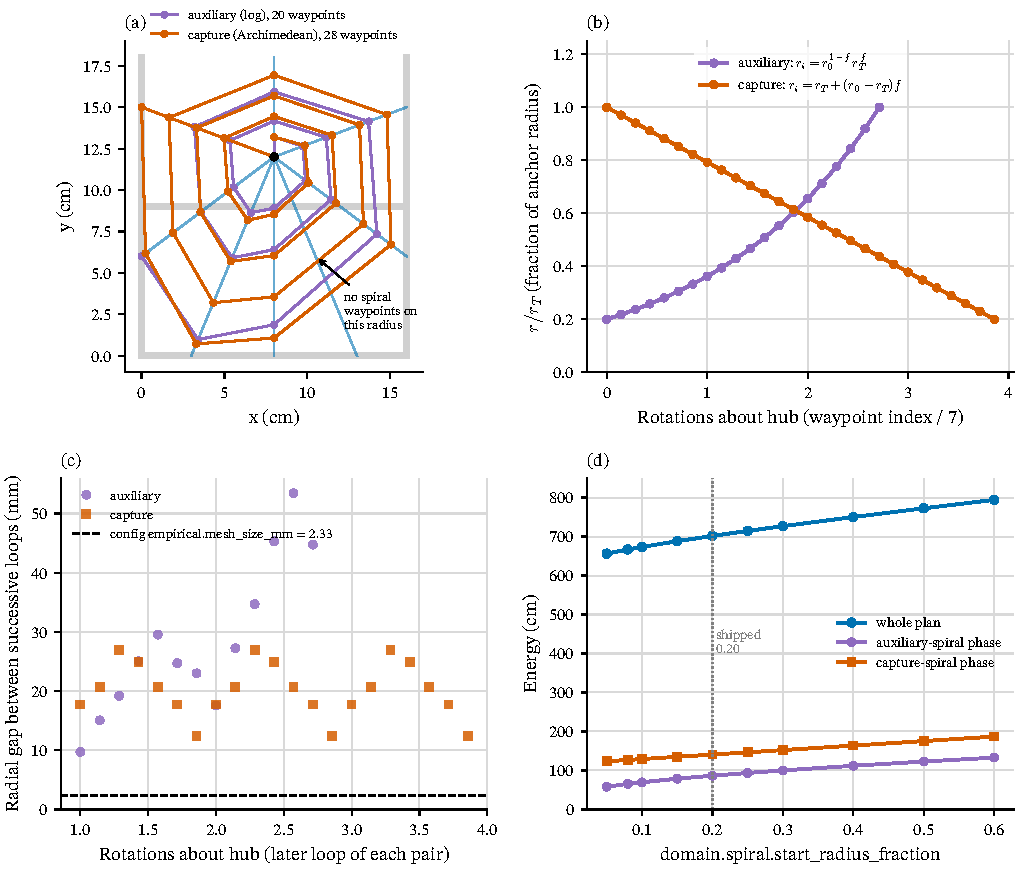
\includegraphics[width=\linewidth]{figures/core/spiral_geometry}
\caption{Spiral geometry generated by \texttt{spiral\_geometry.py} with the shipped \texttt{config.yaml}
(\texttt{61d18d8}). (a) Auxiliary (logarithmic, 20 waypoints) and capture (Archimedean, 28 waypoints)
waypoints with the eight radii; no waypoint lies on the \texttt{anchor\_bottom\_right} radius.
(b) Radius as a fraction of the direction's anchor radius against rotations about the hub
(Eq.~\ref{eq:core-spiral}). (c) Radial gap between successive loops on the same direction, compared with
\texttt{empirical.mesh\_size\_mm}. (d) Total and spiral-phase energy of the deterministic plan against
\texttt{start\_radius\_fraction}; our re-run of the planner for 10 values
(\texttt{scripts/core/rerun\_spiral\_fraction.py}), dotted line at the shipped 0.20.}
\label{fig:core-spiral}
\end{figure}

% =========================================================================================================

\subsection{Configuration, empirical parameters, instrumentation and search strategy}
\label{sec:core-config}

\paragraph{Configuration.} The domain/planner decoupling described in Section 7.1 of the Checkpoint 2
report is in place (\texttt{config.yaml}, \texttt{config\_loader.py}, override via
\texttt{SPIDER\_WEB\_CONFIG}). The configuration now also carries \texttt{domain.spiral}
(Section~\ref{sec:core-spiral}). One status statement needs correcting: at \texttt{39b89f3}, the commit
current when the Checkpoint 2 report was compiled, the shipped \texttt{config.yaml} had
\texttt{stochastic.enabled: true} with anchor removal on ($p=0.2$, seed 7107), so stochasticity was
\emph{not} off by default. It is off by default in \texttt{61d18d8}.

\paragraph{The \texttt{empirical:} block.} \texttt{config.yaml} holds Hesselberg-and-Vollrath-style
figures (web area $239\pm16$\,cm$^2$, radial length $284\pm14$\,cm, capture-spiral length
$1083\pm72$\,cm, mesh size 2.33\,mm, eccentricity 0.47, and Zschokke's median exploration/construction
distances). At \texttt{39b89f3} no code read these values. At \texttt{61d18d8} the efficiency ratio is
implemented as $\eta = S_{\mathrm{used}}/A_{\mathrm{web}}$ (\texttt{utils.efficiency\_ratio}), but
$A_{\mathrm{web}}$ is the convex-hull area of the simulated web's structural nodes
(\texttt{utils.compute\_web\_area}); \texttt{area\_web\_cm2} is only printed by \texttt{compare.py} as an
out-of-scale reference. The empirical figures therefore do not yet ``feed into $\eta$'' as Section 7.3 of
the Checkpoint 2 report states. For the current deterministic plan our re-run of \texttt{compare.py} gives
$A_{\mathrm{web}}=270.0$\,cm$^2$ and $\eta = 701.6/270.0 = 2.60$\,cm\,cm$^{-2}$.

\paragraph{Instrumentation.} \texttt{instrumentation.py} (new) wraps every registered method so that each
decomposition \emph{attempt}, successful or not, increments a counter; \texttt{main.py},
\texttt{sensitivity.py} and \texttt{perturbations.py} report it as the roadmap's ``decomposition depth
$D$'' (a node count, not a recursion depth). For the default plan $D=17$ method calls; the flat baseline
reports $D=0$ by definition.

\paragraph{Search strategy.} Neither package selects a GTPyhop strategy, so both run the installed
default of GTPyhop~1.9.7, iterative greedy search with irrevocable commitment to the first method that
returns a subtask list (recorded in the repository README and in
\texttt{planner\_strategy\_audit.json} under \texttt{docs/research/evidence/}). Algorithm 1 of the Checkpoint 2 report, chronological backtracking on downstream failure,
is therefore not the procedure that ran. In this domain the difference does not change outcomes: re-running
the anchor-removal sweep at \texttt{39b89f3} (9 removal probabilities $\times$ 1000 seeds) with GTPyhop's
explicit \texttt{iterative\_dfs\_backtracking} gave exactly the same success/failure for all 9000 trials
(\texttt{scripts/core/rerun\_htn\_success\_audit.py}). Moreover, the via-drop and via-Tarzan proto-hub
methods never appear in any plan: \textsc{Establish-Proto-Hub-Via-Walk} cycles over eight targets of which
four (stick tops and crossbar ends) are not removable, so it is always applicable. We counted 0
\texttt{drop\_down} and 0 \texttt{swing\_tarzan} actions in 3,819 successful plans at \texttt{39b89f3}
($p\in\{0,0.2,0.5,0.8\}$, 1000 seeds each) and in 1,137 at \texttt{61d18d8} (300 seeds each;
\texttt{scripts/core/rerun\_protohub\_variants.py}). The three-way proto-hub variability is thus encoded
in the method library but is not exercised by any experiment in the repository.

% =========================================================================================================
\FloatBarrier

\subsection{Stochastic layer: anchor removal}
\label{sec:core-anchor}

\texttt{stochastic.py} draws all randomness from one seeded \texttt{random.Random} on the state. Anchor
removal drops each of the eight \texttt{removable\_nodes} independently with probability $p$ before
planning; sticks and crossbars are never removed. The HTN methods are ``best effort'': frame pairs,
radii and spiral spokes whose anchors are missing are skipped. \texttt{sensitivity.py} runs a paired sweep
(same seed per trial for both groups; seeds 1000--1999; baseline step budget 3000). The committed
\texttt{sensitivity\_comparison.csv} covers $p=0$ to $0.8$, not only $0$--$0.5$
(Table~\ref{tab:core-anchor}, Figures~\ref{fig:core-anchor-success}--\ref{fig:core-anchor-energy}).

\paragraph{Reproducibility.} Re-running \texttt{sensitivity.py} at \texttt{39b89f3} for $p\in\{0,0.5,0.8\}$
reproduced every HTN row of the CSV exactly (to all printed digits). The baseline rows did not reproduce
(e.g.\ $p=0$: 967 vs.\ 962 successes, mean 8337 vs.\ 7911\,cm). The cause is in \texttt{baseline.py}:
candidate actions are enumerated from \texttt{list(state.nodes)}, a Python \texttt{set} of strings whose
iteration order depends on the per-process hash seed, so the ``seeded'' walker takes different paths in
different processes unless \texttt{PYTHONHASHSEED} is fixed. This also explains why the $p=0$, $\sigma=0$
baseline row differs between \texttt{sensitivity\_comparison.csv} (962/1000) and
\texttt{wind\_sensitivity.csv} (964/1000), which describe the same condition.

\begin{table}[htbp]
\centering
\caption{Anchor-removal sweep, \texttt{sensitivity\_comparison.csv} (commit \texttt{39b89f3}, wind off,
$n=1000$ trials per group per $p$). Energies are mean $\pm$ SD over successful runs. The last two columns
are our re-run audit at \texttt{39b89f3} with the same seeds: the number of HTN successes whose replayed
plan lays all eight radii (the baseline's \texttt{is\_web\_complete} criterion), and the mean number of
radii in successful HTN plans.}
\label{tab:core-anchor}
\small
\begin{tabular}{rrrrrrrr}
\toprule
$p$ & \multicolumn{2}{c}{Successes / 1000} & \multicolumn{2}{c}{Energy (cm)} & Ratio of & HTN plans & Mean radii \\
\cmidrule(lr){2-3}\cmidrule(lr){4-5}
 & HTN & Baseline & HTN & Baseline & means & with 8 radii & (HTN) \\
\midrule
0.0 & 1000 & 962 & 600.1 $\pm$ 0.0 & 7911 $\pm$ 5613 & 13.2 & 1000 & 8.00 \\
0.1 & 1000 & 961 & 565.8 $\pm$ 42.8 & 7604 $\pm$ 5575 & 13.4 & 426 & 7.21 \\
0.2 & 1000 & 976 & 531.6 $\pm$ 57.2 & 7435 $\pm$ 5715 & 14.0 & 162 & 6.38 \\
0.3 & 1000 & 986 & 498.8 $\pm$ 64.5 & 7098 $\pm$ 5321 & 14.2 & 62 & 5.60 \\
0.4 & 1000 & 992 & 459.9 $\pm$ 70.2 & 6506 $\pm$ 5100 & 14.1 & 16 & 4.74 \\
0.5 & 997 & 993 & 425.0 $\pm$ 71.9 & 6056 $\pm$ 4757 & 14.2 & 3 & 3.95 \\
0.6 & 980 & 992 & 389.3 $\pm$ 70.9 & 5659 $\pm$ 4466 & 14.5 & 0 & 3.16 \\
0.7 & 932 & 998 & 359.1 $\pm$ 66.6 & 5190 $\pm$ 4054 & 14.5 & 0 & 2.52 \\
0.8 & 822 & 999 & 326.8 $\pm$ 57.0 & 4789 $\pm$ 3596 & 14.7 & 0 & 1.88 \\
\bottomrule
\end{tabular}
\end{table}

\paragraph{What the HTN success rate measures.} HTN ``success'' in \texttt{sensitivity.py} means that
\texttt{find\_plan} returned a plan. Our audit shows that the HTN fails exactly when all eight removable
anchors are gone (every one of the 269 failures had zero anchors left, and no trial with zero anchors
succeeded): \textsc{Build-Radii} then has nothing to decompose into. The HTN success probability is
therefore $1-p^8$ (0.996, 0.983, 0.942, 0.832 for $p=0.5$--$0.8$, against observed 0.997, 0.980, 0.932,
0.822). This differs from the explanation in \texttt{insights.md} (the proto-hub gate refusing once fewer
than four anchors remain); the proto-hub step never fails, for the reason given in
Section~\ref{sec:core-config}. Note also that the in-code comments ``require at least 2 frames'' and
``require at least 4 radii'' are not what the code enforces (it only rejects zero).

The two groups are judged by different criteria. A baseline success requires
\texttt{is\_web\_complete}: four frame threads and at least eight radii (between any known nodes, not necessarily
hub and anchor) plus both spiral flags. A best-effort HTN plan under anchor removal lays as many radii as there
are surviving anchors. Already at $p=0.1$ only 42.6\,\% of HTN successes would pass the baseline's
criterion, and none do for $p\ge0.6$ (Figure~\ref{fig:core-anchor-success}b). The opposite trends of the two
success curves (HTN falling, baseline rising from 0.962 to 0.999, crossing between $p=0.5$ and $0.6$) are
therefore not a like-for-like robustness comparison; the baseline's rise reflects that removing anchors
shrinks the set of candidate actions, not that the walker copes better.

\begin{figure}[htbp]
\centering
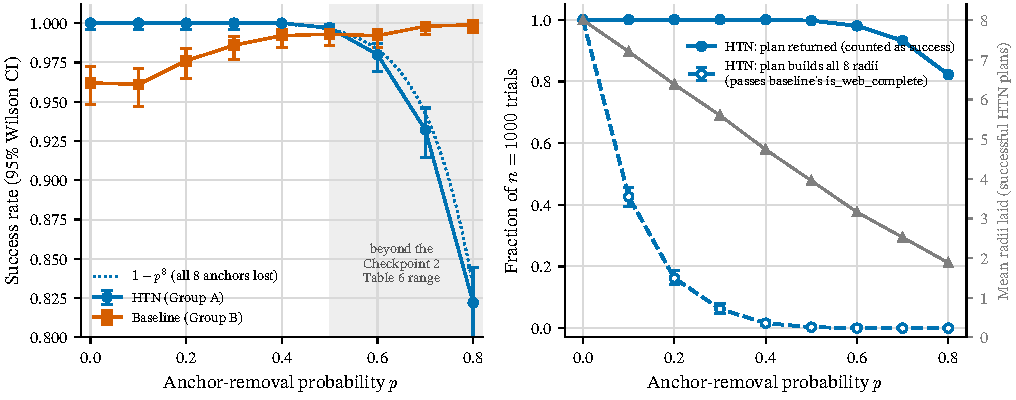
\includegraphics[width=\linewidth]{figures/core/sens_anchor_success}
\caption{(a) Success rate against anchor-removal probability $p$ for the HTN planner and the flat
random-walker baseline (\texttt{sensitivity\_comparison.csv}, \texttt{39b89f3}; $n=1000$ seeded trials
per group per $p$; error bars are 95\,\% Wilson intervals). Dotted: $1-p^8$, the probability that at least
one of the eight removable anchors survives. Shaded: $p>0.5$, outside the range tabulated in the Checkpoint 2
report. (b) Our audit of the HTN runs (re-run at \texttt{39b89f3}, same seeds, $n=1000$ per $p$): fraction
returning a plan, fraction whose plan lays all eight radii (the baseline's completion criterion; Wilson 95\,\%
CI), and mean radii laid by successful plans (right axis).}
\label{fig:core-anchor-success}
\end{figure}

\paragraph{Energy.} HTN energy falls from 600.1\,cm at $p=0$ to 326.8\,cm at $p=0.8$ because a web with
fewer anchors has fewer radii and spiral spokes; the HTN's dispersion comes entirely from which anchors
were drawn. The baseline's energy also falls (7911\,$\to$\,4789\,cm) but its SD stays at 71--79\,\% of the
mean. The ratio of mean energies lies between 13.2 and 14.7 at every $p$, and the ratio of medians between
10.3 and 11.5 (Figure~\ref{fig:core-anchor-energy}). This order-of-magnitude gap is the most stable number
in the sweep, but it compares a fixed procedure that knows the construction order with an uninformed
random walker over the same operators; it shows how much the encoded order saves relative to undirected
search, not that hierarchical control is necessary.

\begin{figure}[htbp]
\centering
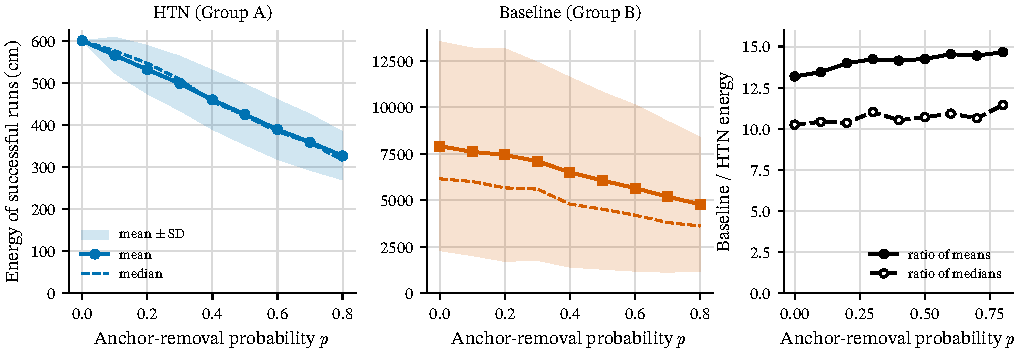
\includegraphics[width=\linewidth]{figures/core/sens_anchor_energy}
\caption{Locomotory energy of successful runs against anchor-removal probability: HTN (left) and baseline
(middle), mean (markers), $\pm$1 SD (band) and median (dashed); right: baseline/HTN ratio of means and of
medians. Source: \texttt{sensitivity\_comparison.csv} (\texttt{39b89f3}), $n=1000$ trials per group per
$p$ (successful runs only; see Table~\ref{tab:core-anchor} for counts).}
\label{fig:core-anchor-energy}
\end{figure}

% =========================================================================================================

\subsection{Stochastic layer: wind}
\label{sec:core-wind}

Table 4 of the Checkpoint 2 report lists the sweep as ``wind currently off''. A wind sweep had in fact been
run and committed before that report (\texttt{wind\_sensitivity.csv}, \texttt{39b89f3}, 2026-09-09). Wind
multiplies every movement cost by $\max(1+\varepsilon, 0.1)$ with $\varepsilon\sim\mathcal{N}(0,\sigma^2)$
drawn per step; the sweep holds $p=0$ and takes $\sigma\in\{0,0.05,\dots,0.3,0.4,0.5\}$ with 1000 trials
per group (Figure~\ref{fig:core-wind}). We re-ran $\sigma\in\{0,0.5\}$ at \texttt{39b89f3}: the HTN rows
reproduced exactly; the baseline rows again did not (hash-seed dependence, Section~\ref{sec:core-anchor}).

\begin{itemize}
  \item \textbf{Success is unaffected for both groups} (HTN 1000/1000, baseline 964/1000 at every
  $\sigma$). No operator precondition reads a cost or \texttt{energy\_expended} (\texttt{insights.md}
  documents this check), so wind can only change the reported cost. The baseline's count is identical at
  every $\sigma$ because its action choices come from a separate RNG; wind rescales the same trajectories.
  \item \textbf{HTN energy SD grows linearly}: SD$/\sigma = 81.6$\,cm for $\sigma\le0.25$ (81.6, 80.9 and
  79.5 at 0.3, 0.4, 0.5), i.e.\ the root sum of squared step lengths of the fixed plan, as expected for
  independent per-step noise.
  \item \textbf{HTN mean energy} stays at 600.1--600.2\,cm up to $\sigma=0.3$ and rises to 604.7\,cm at
  $\sigma=0.5$. This rise is the bias introduced by the 0.1 floor: the analytic expectation
  $E_0\,\mathbb{E}[\max(1+\varepsilon,0.1)]$ gives 604.4\,cm at $\sigma=0.5$ (dotted curve).
  \item \textbf{Baseline} mean and median rise by less than 1\,\% (8224\,$\to$\,8294\,cm, median
  6443\,$\to$\,6518\,cm); its SD (6045--6102\,cm) is dominated by path randomness, not wind.
\end{itemize}
The CSV is the ``corrected'' sweep of \texttt{insights.md}: an earlier version re-drew wind noise from
the RNG left over after GTPyhop's search, producing a spurious upward drift (600.1\,$\to$\,605.9\,cm); the fix
executes the found plan once on a fresh state with a dedicated per-trial RNG. Within this model wind is
a measurement perturbation, not a hazard: there is no energy budget or thread breakage that it could
trigger (the silk-capacity mechanism of Section~\ref{sec:core-perturb} is not active in these sweeps).

\begin{figure}[htbp]
\centering
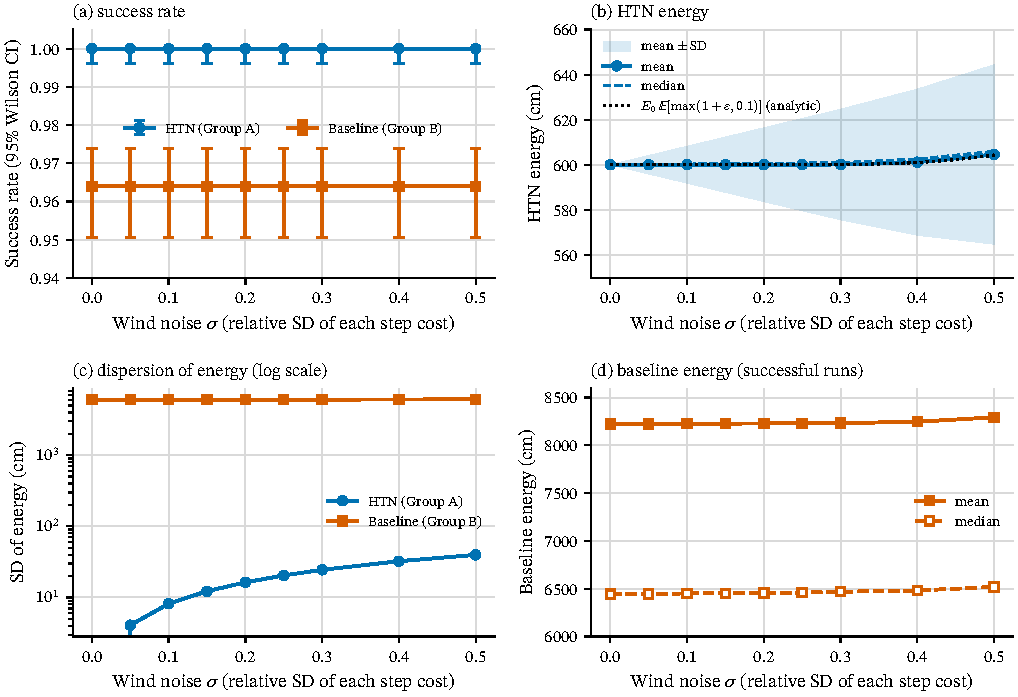
\includegraphics[width=\linewidth]{figures/core/wind_sensitivity}
\caption{Wind-noise sweep, all metrics of \texttt{wind\_sensitivity.csv} (\texttt{39b89f3}; anchor
removal off; $n=1000$ trials per group per $\sigma$). (a) Success rate with 95\,\% Wilson intervals.
(b) HTN energy: mean, $\pm$1 SD band and median; dotted, the analytic mean implied by the clamped
multiplier (computed by us, not in the repository). (c) SD of energy, both groups, log scale ($\sigma=0$
omitted for the HTN, SD $=0$). (d) Baseline mean and median energy of successful runs.}
\label{fig:core-wind}
\end{figure}

% =========================================================================================================
\FloatBarrier

\subsection{HTN versus the flat random-walker baseline}
\label{sec:core-compare}

\texttt{baseline.py} (Group B) is a seeded random walker over the HTN's own operators. At each step it
enumerates ``structurally plausible'' candidates (walks to neighbours, threads from the current node to
every known node, and, once a proto-hub exists, frame/radius/spiral segments to every known node plus the
two spiral-done markers) and picks one uniformly; operator preconditions decide legality. Its success
criterion \texttt{is\_web\_complete} counts frames, radii and flags but not geometry: the spiral flags can
be set without laying spiral silk (in our 300-seed re-run, one successful walker laid no capture-spiral
segment), and a ``radius'' may be laid between any two known nodes (the walker calls
\texttt{lay\_radius} with its current position as the hub argument). \texttt{compare.py} runs the deterministic HTN plan once
and the walker over $n$ seeds.

\paragraph{The Checkpoint 2 Table 5 numbers.} The HTN entry there (61 actions, 524.8\,cm) equals
\texttt{single\_run\_comparison.csv} and our re-run of \texttt{compare.py} at \texttt{39b89f3}. It is not a
run ``with anchor removal and wind off'': the shipped configuration had anchor removal on, and the HTN run
used the configured seed 7107, which removes \texttt{anchor\_top\_center}, \texttt{anchor\_bottom\_center}
and \texttt{anchor\_bottom\_right} (five radii instead of eight). The deterministic Checkpoint 2 plan is the
71-action, 600.1\,cm plan of Table~\ref{tab:core-phases}, which is also the HTN value at $p=0$ in
Table~\ref{tab:core-anchor}; quoting 524.8\,cm and 600.1\,cm as the same plan is inconsistent. The baseline
entry ($0.97$, $7492.3\pm6370.5$\,cm, $\sim$750 actions) could not be reproduced:
\texttt{single\_run\_comparison.csv} itself holds a different baseline result (769 actions, 7711.4\,cm,
success 1.0), and re-running \texttt{compare.py} at \texttt{39b89f3} (30 seeds, 5000 steps) under ten
values of \texttt{PYTHONHASHSEED} gave success 1.00 every time and 30-seed mean energies from 5836 to
10781\,cm (Figure~\ref{fig:core-compare}b). A 30-seed summary of this walker is therefore not a stable
quantity, and it depends on an uncontrolled process setting.

\paragraph{Current comparison.} Table~\ref{tab:core-compare} and Figures~\ref{fig:core-compare} and
\ref{fig:core-compare-dist} report our re-run of \texttt{compare.py} at \texttt{61d18d8} with 300 walker
seeds (5000-step budget, \texttt{PYTHONHASHSEED=0}). The walker succeeded in 299 of 300 runs; its energy
has median 6186\,cm and a long right tail (944--34{,}016\,cm), against the HTN's deterministic 701.6\,cm.
No walker run used less energy than the HTN plan (minimum ratio 1.35), although the shortest walker run
needed fewer action attempts (94) than the HTN plan has actions (105), which is possible only because the
walker's criterion does not require a full spiral.

\begin{table}[htbp]
\centering
\caption{HTN (Group A) vs.\ flat random walker (Group B): our re-run of \texttt{compare.py} at
\texttt{61d18d8} (shipped deterministic config, 300 walker seeds, 5000-step budget,
\texttt{PYTHONHASHSEED=0}; scripts \texttt{rerun\_compare.py}, \texttt{rerun\_checks.sh}). Walker statistics
over its 299 successful runs. $\eta$ uses the convex-hull area of each simulated web.}
\label{tab:core-compare}
\small
\begin{tabular}{lrr}
\toprule
Metric & HTN (Group A) & Random walker (Group B) \\
\midrule
Success & 1 plan (deterministic) & 299/300 (0.997) \\
Energy (cm) & 701.6 & mean 8188.8 $\pm$ 6273.6 (SD); median 6185.8 \\
Actions / action attempts & 105 & mean 822; median 591; min 94 \\
Efficiency $\eta$ (cm\,cm$^{-2}$) & 2.60 ($A_{\mathrm{web}}=270.0$\,cm$^2$) & mean 28.4 \\
Decomposition count $D$ & 17 & 0 (no hierarchy) \\
\bottomrule
\end{tabular}
\end{table}

\begin{figure}[htbp]
\centering
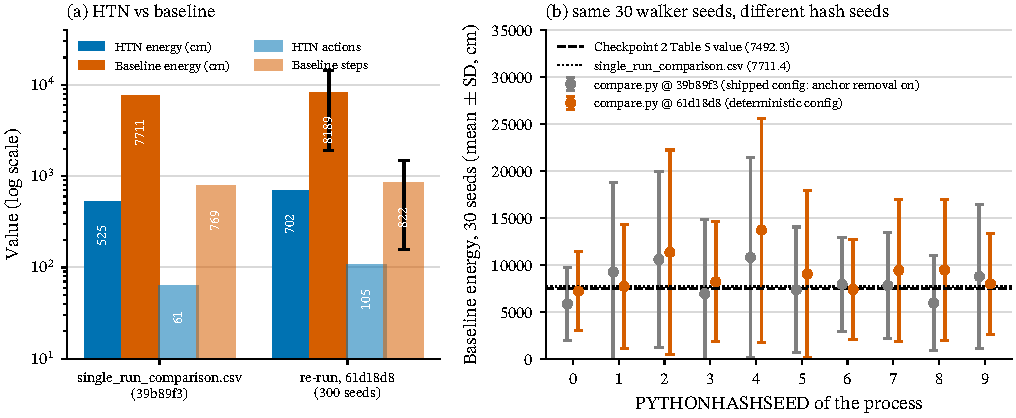
\includegraphics[width=\linewidth]{figures/core/compare_summary}
\caption{(a) HTN vs.\ baseline energy and action/step counts on a log scale: \texttt{single\_run\_comparison.csv}
(\texttt{39b89f3}; HTN run with anchor removal on, seed 7107) and our 300-seed re-run at \texttt{61d18d8}
(error bars: SD over 299 successful walker runs). (b) Baseline 30-seed mean energy $\pm$ SD from
\texttt{compare.py} re-run with the same 30 walker seeds under ten values of \texttt{PYTHONHASHSEED}, at
\texttt{39b89f3} (shipped config) and \texttt{61d18d8} (deterministic config); horizontal lines: the
Checkpoint 2 Table 5 value and the committed CSV value.}
\label{fig:core-compare}
\end{figure}

\begin{figure}[htbp]
\centering
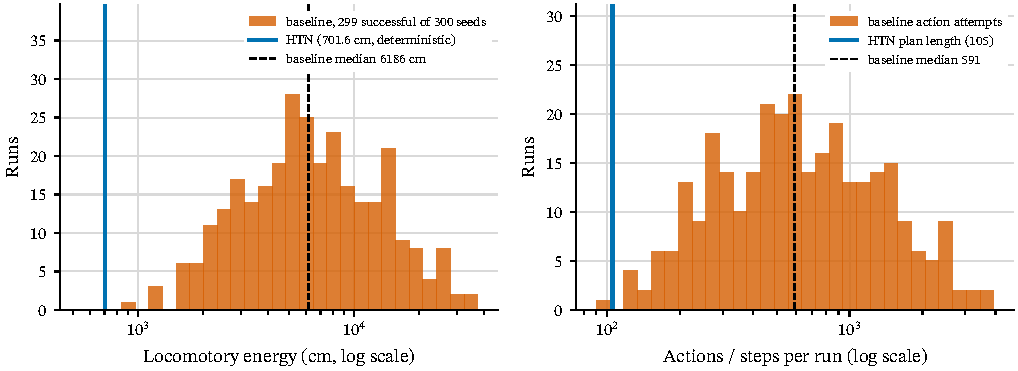
\includegraphics[width=\linewidth]{figures/core/compare_distributions}
\caption{Per-seed distributions from our re-run of \texttt{compare.py} at \texttt{61d18d8} (300 seeds,
\texttt{PYTHONHASHSEED=0}; 299 successful walker runs shown): locomotory energy (left) and action attempts
(right), log axes, with the deterministic HTN value (blue) and the walker median (dashed).}
\label{fig:core-compare-dist}
\end{figure}

% =========================================================================================================

\subsection{Adaptive replanning and perturbation trials (historical, unaudited)}
\label{sec:core-perturb}

Commit \texttt{61d18d8} restored from a local stash an adaptive-planner extension of the updated package:
\texttt{perturbations.py} and its output \texttt{perturbation\_trials.csv}, together with
\texttt{silk\_capacity} and \texttt{predator\_present} state fields, a capacity check in every movement
operator, a \texttt{flee\_from\_predator} operator (3\,cm) and a predator check at the top of
\textsc{Build-Web}. The claim ledger is explicit (C28): the CSV and code were recovered without a
contemporaneous provenance manifest, so the CSV is \emph{historical, unaudited output}, and it does not
establish an HTN advantage. We describe the design and the numbers on that basis only.

\paragraph{Design.} Three stressors fire once, right after the proto-hub is established, in both groups:
\emph{resource depletion} cuts the remaining silk budget by 30\,\% (initial capacity 2200\,cm);
\emph{structural failure} deletes a random anchor already carrying a frame, radius or proto-radius, with its
threads and progress counters; \emph{predator} forces a flee before construction resumes. The HTN replays its
plan up to the trigger, applies the perturbation and calls \texttt{find\_plan} again from the live state;
this is fresh re-planning from the root task, not repair of a retained decomposition tree. Adaptation time
$T_a$ is the HTN continuation length minus the undisturbed remainder, and for the walker the number of
steps from trigger to completion.

\paragraph{Numbers and caveats.} The CSV reports HTN success 200/200 for every stressor
(energy 701.6, 638.3, 704.6\,cm; $T_a = 0$, $-11.8$, $+1$) and walker success 36, 44 and 46 of 200
(Figure~\ref{fig:core-perturb}). Our re-run of the module with its default settings at \texttt{61d18d8}
reproduced the HTN rows exactly and gave walker successes of 40, 45 and 49 (the same hash-seed effect).
The work log's one-seed smoke check is software verification, and so is ours; neither is an audit. Three
features of the design limit what the numbers can mean: (i) the HTN is deterministic under the shipped
config, so its 200 trials per stressor are one trial repeated (SD of $T_a$ is 0 except for structural
failure, where only the destroyed anchor varies); (ii) the walker's typical unperturbed energy (median
6186\,cm, Table~\ref{tab:core-compare}) is about three times the 2200\,cm silk cap, so most walker
failures are budget exhaustion and the successful walker runs are the short ones (mean energies
1760--1979\,cm, just under the cap); (iii) $T_a$ is counted in plan actions for the HTN and in action
attempts for the walker, and the HTN's negative $T_a$ under structural failure means it builds less web
after losing an anchor, not that it recovers faster. A fair test of replanning would need an
equal-exposure design, a budget scaled to each agent, and a structural completion check for both groups.

\begin{figure}[htbp]
\centering
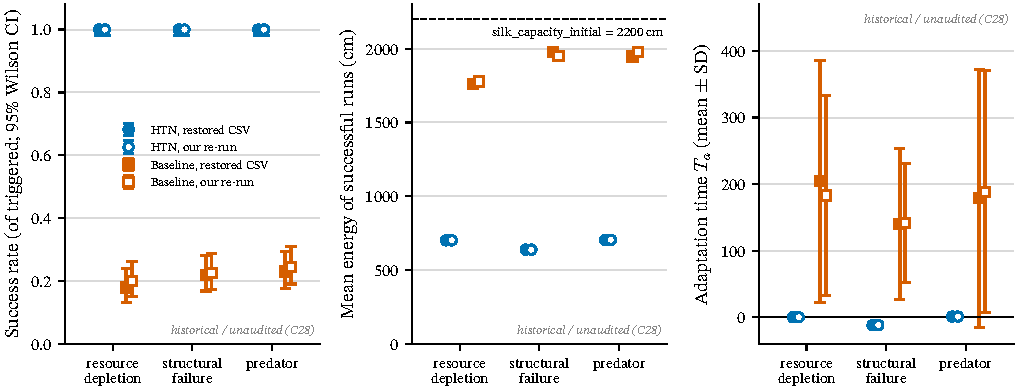
\includegraphics[width=\linewidth]{figures/core/perturbation_trials_historical}
\caption{\emph{Historical, unaudited output (claim C28).} Restored \texttt{perturbation\_trials.csv}
(filled markers; $n=200$ trials per group per stressor, all triggered) and our default-settings re-run of
\texttt{perturbations.py} at \texttt{61d18d8} (open markers). Left: success rate over triggered trials,
95\,\% Wilson intervals; middle: mean energy of successful runs, dashed line the initial silk capacity;
right: adaptation time $T_a$, mean $\pm$ SD (units differ between groups, see text). Shown for completeness;
not evidence for an HTN advantage.}
\label{fig:core-perturb}
\end{figure}

% =========================================================================================================

\subsection{Test suite}
\label{sec:core-tests}

Running \texttt{pytest} in \texttt{spider\_web\_htn\_updated/} in a private checkout gives 56 tests in
5 files at \texttt{61d18d8}, all passing (55 at \texttt{39b89f3}, also all passing;
Figure~\ref{fig:core-tests}). The one new test checks that a spiral segment refused for lack of silk
capacity leaves the state unmodified. The deterministic regression target in \texttt{test\_planner.py}
moved from 71 actions / 600.1\,cm to 105 actions / 701.6\,cm with the new spiral geometry. Two limits are
worth stating. First, \texttt{perturbations.py}, \texttt{sensitivity.py}, \texttt{compare.py},
\texttt{instrumentation.py} and \texttt{spiral\_geometry.py} have no direct tests; the spiral code is covered
only through the regression totals. Second, Section 7.2 of the Checkpoint 2 report says the suite verifies
that ``no spiral-laying operator can fire before the bridge and proto-hub''; \texttt{build\_spiral\_segment}
has no such precondition (it checks only the spider's position, anchor availability and, now, silk
capacity), and the corresponding test (\texttt{test\_enumerate\_candidate\_actions\_gates\_later\_stages\_behind\_proto\_hub})
concerns the baseline's candidate list. The ordering is enforced by the HTN methods, not by the operators.
The repository-wide figure of 177 passing tests in the work log includes the Mulder and recovery suites.

\begin{figure}[htbp]
\centering
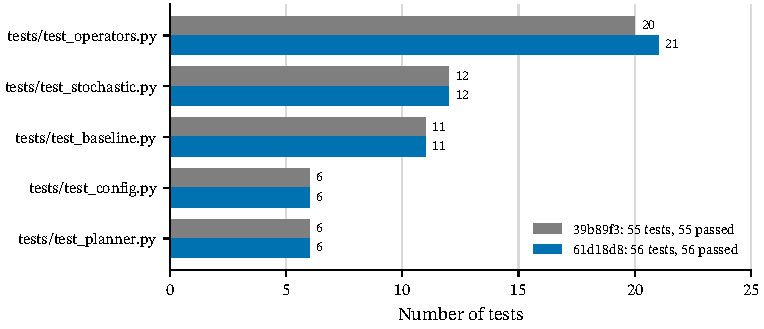
\includegraphics[width=0.72\linewidth]{figures/core/tests_per_file}
\caption{Tests per file in \texttt{spider\_web\_htn\_updated/tests}, from our \texttt{pytest} runs
(junit XML) in private checkouts at \texttt{39b89f3} (55 tests) and \texttt{61d18d8} (56 tests); all
passed in both.}
\label{fig:core-tests}
\end{figure}

% =========================================================================================================
\FloatBarrier

\subsection{Corrections to the Checkpoint 2 report}
\label{sec:core-corrections}

Table~\ref{tab:core-corrections} collects the statements of the Checkpoint 2 report that the
sections above correct, each with its evidence.

\begin{table}[htbp]
\centering
\caption{Statements in Sections 6--9 of the Checkpoint 2 report that the repository contradicts or has
superseded, with the corrected statement and its evidence.}\label{tab:core-corrections}
\small
\begin{tabular}{>{\raggedright\arraybackslash}p{0.30\linewidth}>{\raggedright\arraybackslash}p{0.64\linewidth}}
\toprule
Checkpoint 2 statement & Correction (evidence) \\
\midrule
Default plan has 70 actions (Fig.~1, Table 3) & The plan whose energies are quoted has 71 actions (exploration 10), per its own regression test and our re-export at \texttt{39b89f3}. The current updated plan has 105 actions, 701.6\,cm; the original package 128 actions, 751.6\,cm. \\
\addlinespace[3pt]
Fig.~1 shows the interactive visualiser's final state & The committed \texttt{index.html} plays the original package's 128-action plan; no committed data file yields the 70-action view. \\
\addlinespace[3pt]
Algorithm 8 / Table 2: spirals as Archimedean traversal / ``1 loop over the 8 radii anchors'' & Algorithm 8 describes the original package; the 600.1\,cm numbers came from the updated package, whose spirals were then one pass through 7 boundary anchors. Now: log auxiliary + Archimedean capture waypoints, 2.71 and 3.86 rotations over 7 directions (Section~\ref{sec:core-spiral}). \\
\addlinespace[3pt]
Spiral phases are shallow (10.4\,\% each) & True only of the heptagon placeholder; now 12.3\,\% and 20.0\,\%. \\
\addlinespace[3pt]
Algorithm 1: chronological backtracking; three proto-hub strategies explored & Installed GTPyhop default is greedy without backtracking (outcome-identical in our 9000-trial check); via-drop and via-Tarzan never occur in any plan. \\
\addlinespace[3pt]
Stochasticity off by default (Table 4, \S7.6) & At \texttt{39b89f3} the shipped config had anchor removal on ($p=0.2$, seed 7107); off by default only since \texttt{61d18d8}. \\
\addlinespace[3pt]
Sensitivity sweep ``wind currently off'' (Table 4) & \texttt{wind\_sensitivity.csv} ($\sigma$ up to 0.5, $n=1000$) was committed on 2026-09-09, before the report (Section~\ref{sec:core-wind}). \\
\addlinespace[3pt]
Sweep from 0\,\% to 50\,\%; HTN 1.00 throughout; baseline never closes the gap & CSV runs to 80\,\%; HTN 0.997 at 50\,\%, 0.980, 0.932, 0.822 at 60--80\,\%; baseline exceeds HTN from 60\,\%. Success criteria differ between groups (Section~\ref{sec:core-anchor}). \\
\addlinespace[3pt]
Table 6 baseline 0.98 at 10\,\% and 30\,\% & CSV: 0.961 and 0.986. \\
\addlinespace[3pt]
Baseline energy falls 8{,}239\,$\to$\,5{,}876\,cm & CSV: 7911.4\,$\to$\,6055.9\,cm ($p=0\to0.5$). \\
\addlinespace[3pt]
Table 5: HTN 524.8\,cm, 61 actions, ``anchor removal and wind off'' & That run had anchor removal on (seed 7107, three anchors removed). The wind-free, removal-free plan is 600.1\,cm (71 actions), the value used elsewhere in the same report. \\
\addlinespace[3pt]
Table 5: baseline $0.97$, $7492.3\pm6370.5$\,cm, $\sim$750 actions; ``14.3$\times$'' & Not reproducible; \texttt{single\_run\_comparison.csv} has 769 actions, 7711.4\,cm; walker results depend on \texttt{PYTHONHASHSEED} (30-seed means 5836--10781\,cm at \texttt{39b89f3}). Ratio of means in the 1000-trial sweep: 13.2--14.7; of medians 10.3--11.5. \\
\addlinespace[3pt]
Empirical block wired into $\eta$ (\S7.3) & Not read by any computation; $\eta$ uses the simulated web's convex-hull area (2.60\,cm\,cm$^{-2}$ for the current plan). \\
\addlinespace[3pt]
5 test files, 55 tests (\S7.2) & 55 was correct at \texttt{39b89f3}; now 56 in 5 files, all passing. The operator-level spiral gating claimed in \S7.2 does not exist. \\
\bottomrule
\end{tabular}
\end{table}
\FloatBarrier
